\documentclass[10pt,a4paper,final]{report}
\usepackage[latin1]{inputenc}
\usepackage{amsmath}
\usepackage{amsfonts}
\usepackage{amssymb}
\usepackage{graphicx}
\usepackage{listings}
\usepackage{comment}

\title{Miniproject 1 - DIS}
\author{Lars Andersen, Mathias Winde Pedersen \& S�ren Skibsted Als}
\begin{document}
	\maketitle
	\begin{comment}

	\section*{B}
	By looking at the data, different business processes have been considered.
	A central one is that of sale.
	Another process to model is the payment process, which is the pre-insertion of money.
	
	We choose to focus on the sale business process.
	
	For the granularity, the data already contains a timestamp for each sale, as of such we maintain that granularity.
	
	
	That is timestamp without timezone, containing year, month, day, hour, minute and second.
	However, a weekday could be relevant as well, and when extracting the data, it could be interesting to include this information, same goes for season, holidays, and week number.
	
	The granularity for a member is year, as we cannot go deeper there, without coming up with some fictive data.
	
	The choices are reasonable for paying customers, which is reflected in the questions that can be asked.
	
	For sales, it could be interesting to see if the sales increase during breaks, and the granularity here is fine with down to minutes, for seconds it is still fine as it does not require much effort to record this as well.
	
	For member creation the year of creation is as close as we can get, thus this is also reasonable for the given data.
	
	\textbf{Questions that can be asked:}
	
	Does sales increase during break times (12:00 to 12:30)?
	
	How has the total sales per year evolved?
	
	Which product has been sold the most?
	
	Which member spends the most money?
	
	Which weekday, weeknumber, season, holiday have the largest revenue?
	
	
	\section*{C}
	For SCDs products could be useful, as the price changes slowly over time, same goes for members, as they can be active or inactive.
	
	For the time dimension, we skipped weekdays etc. as we would have to find a library of some sort to translate this.
	The dimensions have been specified in Figure \ref{fig:dimensions}. The schema can be seen in the code below and in Figure \ref{fig:schema}.
	
	\begin{figure}[h]
		\centering
		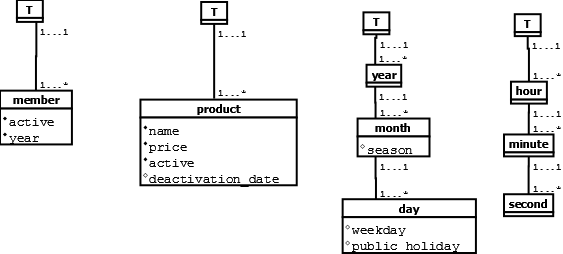
\includegraphics[scale=0.5]{dimensions}
		\caption{Dimensions, part C.}
		\label{fig:dimensions}
	\end{figure}
	
	\newpage
	\lstinputlisting[language=SQL]{codeschema.txt}
	
	\begin{figure}[h]
		\centering
		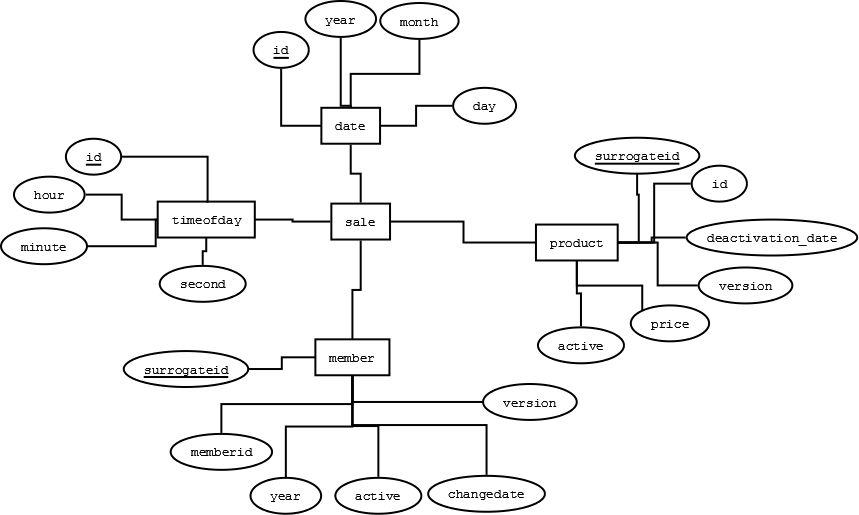
\includegraphics[scale=0.3]{starscheme}
		\caption{schema, part C.}
		\label{fig:schema}
	\end{figure}
	\newpage
		\end{comment}
	
	\section*{D}
	We started this exercise with an overall plan, where we decided to load the data from the database, and then to transform this data and insert it into the dimension tables.
	After this, the fact table can be filled.
	We realised that the schema had to be changed, and as of such we moved the price from the dimension product, to the fact table, as price is what we measure.
	Additionally, we do not have incremental loads, but should be strived for in a larger and more permanent system.
	
	In figure \ref{fig:filldimensions} a flow of how the dimensions are filled can be seen.
	\begin{figure}[h]
		\centering
		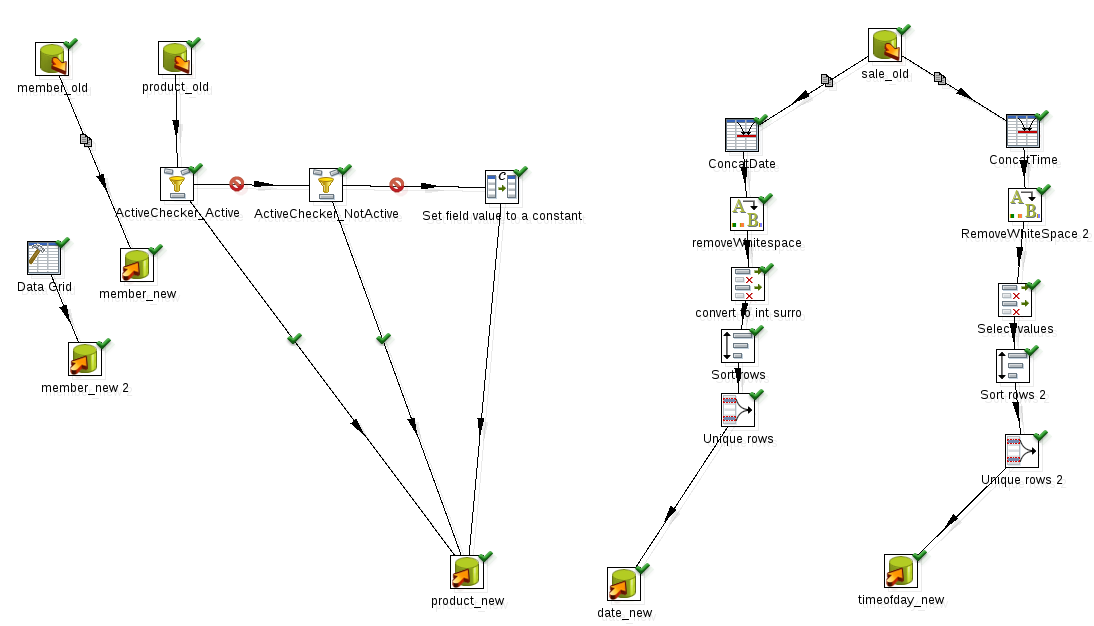
\includegraphics[scale=0.5]{filldimensions}
		\caption{Flow for filling of dimensions}
		\label{fig:filldimensions}
	\end{figure}
	As can be seen, members are added straightforward, as the old and new database map one to one, with just an additional surrogate key.
	However, a dirty fix is that we add a member with memberid -1, in order to handle an error that occurred when filling the fact table (more on this in the description of the fact table flow).
	
	The filling of the product is straight forward too, but we do some datacleaning, as some product were active but had a deactivation date, this data got deactivated instead.
	
	For the filling of the date and timeofday dimension, it gets a bit more complicated. What we do there is to extract the information (year, month, day, hour, minute, second).
	When this is done, we generate a primary key by concatenating the information. So for date the primary key consists of year month day, and then for timeofday it is hour minute second.

	In figure \ref{fig:fillfact}, the flow for filling the fact table can be seen.
	\begin{figure}[h]
		\centering
		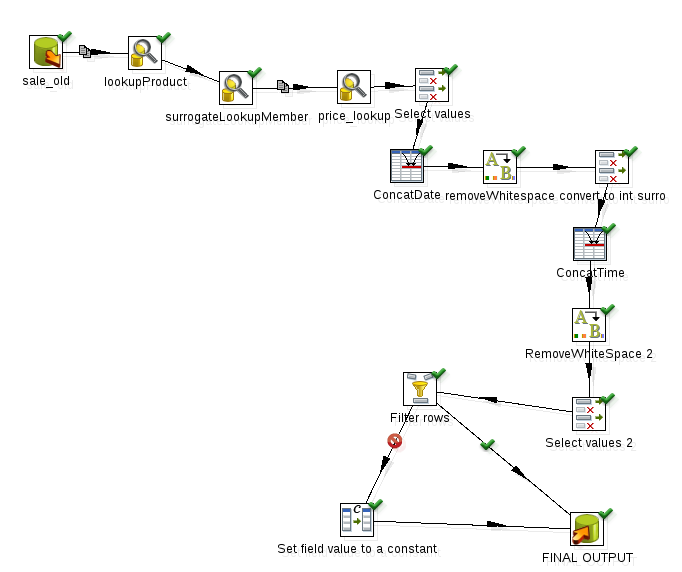
\includegraphics[scale=0.8]{fillfacttable}
		\caption{Flow for filling the fact table}
		\label{fig:fillfact}
	\end{figure}
	The figure depicts how the various surrogatekeys gets looked up in the dimension tables, as well as the price which is looked up in the old product table.
	After the lookups, the same generation of surrogate keys as in the filling of date and time dimensions are used, to get the same keys.
	Lastly, the mentioned erroneous memberids are filtered, such that members with an invalid memberid(0) gets changed to -1.
		
\end{document}